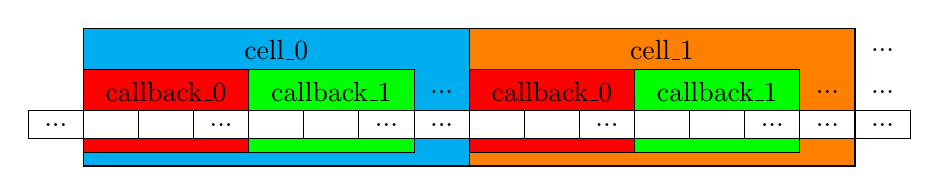
\begin{tikzpicture}[scale=0.7]
  % draw cells
  \draw[fill=cyan] (0,-0.5) rectangle ( 7,2);
  \draw[fill=orange]    (7,-0.5) rectangle (14,2);
  \node[align=center] at ( 3.5, 1.6) {cell\textunderscore{}0};
  \node[align=center] at (10.5, 1.6) {cell\textunderscore{}1};
  \node[align=center] at (14.5, 1.6) {...};
  
  % draw callbacks
  % cell_1
  \draw[fill=red]   (0,-0.25) rectangle (3,1.25);
  \draw[fill=green] (3,-0.25) rectangle (6,1.25);
  \node[align=center] at (1.5,0.85) {callback\textunderscore{}0};
  \node[align=center] at (4.5,0.85) {callback\textunderscore{}1};
  \node[align=center] at (6.5,0.85) {...};
  % cell_2
  \draw[fill=red]   ( 7,-0.25) rectangle (10,1.25);
  \draw[fill=green] (10,-0.25) rectangle (13,1.25);
  \node[align=center] at ( 8.5,0.85) {callback\textunderscore{}0};
  \node[align=center] at (11.5,0.85) {callback\textunderscore{}1};
  \node[align=center] at (13.5,0.85) {...};
  % beyond
  \node[align=center] at (14.5,0.85) {...};
  
  % draw contiguous memory
  \draw[fill=white] (-1,0) rectangle (15,0.5);
  \foreach \x in {0,...,14}
  \draw (\x,0) -- (\x,0.5);
  % cell_1
  \node[align=center] at ( 2.5,0.25) {...};
  \node[align=center] at ( 5.5,0.25) {...};
  \node[align=center] at ( 6.5,0.25) {...};
  % cell_2
  \node[align=center] at ( 9.5,0.25) {...};
  \node[align=center] at (12.5,0.25) {...};
  \node[align=center] at (13.5,0.25) {...};
  % beyond
  \node[align=center] at (-0.5,0.25) {...};
  \node[align=center] at (14.5,0.25) {...};
\end{tikzpicture}